\documentclass[convert]{standalone}

\usepackage{tikz}
\usetikzlibrary{calc}
\begin{document}
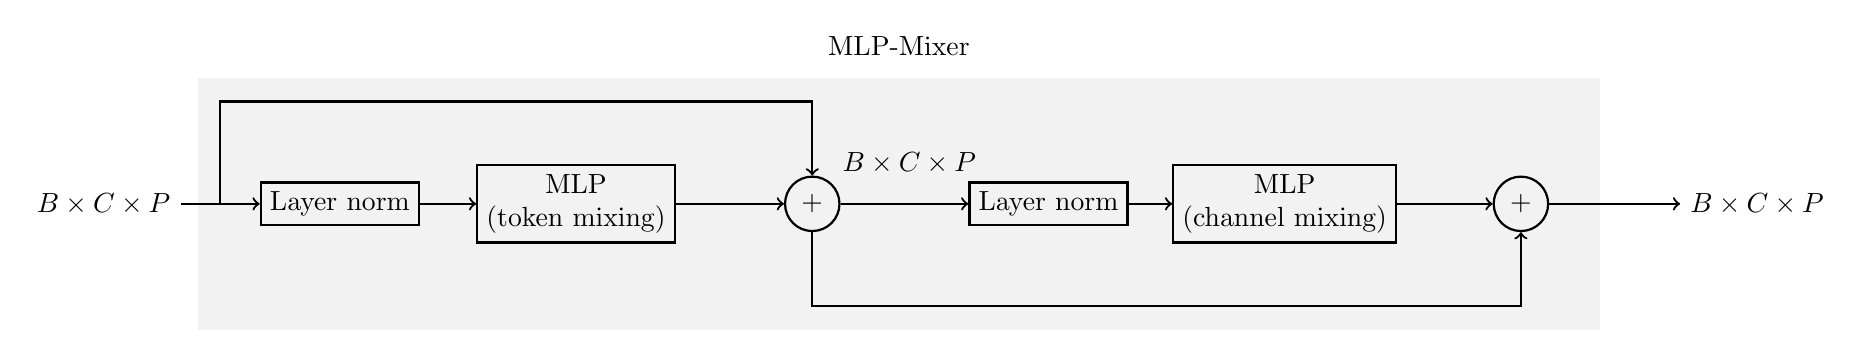
\begin{tikzpicture}[node distance=3cm, thick]
    \fill[gray!10] (1.2cm, 1.6cm) rectangle (19cm, -1.6cm);
    \node at (10.1cm, 2cm) {MLP-Mixer};
    \node at (0, 0) (input){$B \times C \times P$};
    \node[right of=input, shape=rectangle, draw] (ln1) {Layer norm};
    \node[right of=ln1, shape=rectangle, draw, align=center] (mlp1) {MLP\\ (token mixing)};
    \node[right of=mlp1, shape=circle, draw, label={45:$B \times C \times P$}] (plus1) {+};
    \node[right of=plus1, shape=rectangle, draw] (ln2) {Layer norm};
    \node[right of=ln2, shape=rectangle, draw, align=center] (mlp2) {MLP\\ (channel mixing)};
    \node[right of=mlp2, shape=circle, draw] (plus2) {+};
    \node[right of=plus2] (output){$B \times C \times P$};
    \draw[->] (input) -- (ln1);
    \draw[->] (ln1) -- (mlp1);
    \draw[->] (mlp1) -- (plus1);
    \draw[->] (plus1) -- (ln2);
    \draw[->] (ln2) -- (mlp2);
    \draw[->] (mlp2) -- (plus2);
    \draw[->] (plus2) -- (output);
    \draw[->] ($(input.east) + (0.5cm, 0)$) -- ++(0, 1.3cm) -| (plus1);
    \draw[->] (plus1) -- ++(0, -1.3cm) -| (plus2);
\end{tikzpicture}
\end{document}
